\documentclass[11pt,a4paper]{article}
\usepackage[utf8]{inputenc}
\usepackage[T1]{fontenc}
\usepackage[italian]{babel}
\usepackage{lmodern}
\usepackage[a4paper,margin=2cm]{geometry}
\usepackage{graphicx,booktabs,tabularx,longtable,array,enumitem,xcolor,hyperref,fancyhdr,microtype,lastpage}
\definecolor{accent}{HTML}{17365D}
\definecolor{warn}{HTML}{8A5A00}
\definecolor{ok}{HTML}{245B38}
\hypersetup{colorlinks=true,linkcolor=accent,urlcolor=accent,pdftitle={Dossier urbanistico-catastale - Via Fausto Bufalini 23, Messina}}
\pagestyle{fancy}\fancyhf{}\lhead{\small Via Fausto Bufalini 23 -- Messina}\rhead{\small Dossier incrementale}\cfoot{\small Pagina \thepage\ di \pageref{LastPage}}
\setlength{\parindent}{0pt}\setlength{\parskip}{5pt}\renewcommand{\arraystretch}{1.16}
\newcommand{\docu}[1]{\textbf{\color{ok}Documentato:} #1}
\newcommand{\memo}[1]{\textbf{\color{accent}Ricordo/testimonianza:} #1}
\newcommand{\infer}[1]{\textbf{\color{warn}Inferenza:} #1}
\newcommand{\openq}[1]{\textbf{\color{warn}Questione aperta:} #1}
\begin{document}
\begin{titlepage}\centering\vspace*{2cm}
{\Huge\bfseries Dossier urbanistico-catastale\par}\vspace{.5cm}
{\LARGE Via Fausto Bufalini 23 -- Messina\par}\vspace{.8cm}
{\large Foglio 124 -- Particella 509 -- Subalterno 5\par}
\vfill
\begin{minipage}{.82\textwidth}\centering\itshape
Documento di lavoro incrementale per ricostruire la storia catastale e urbanistica dell'unità e del fabbricato prima di un eventuale accesso agli atti comunale.
\end{minipage}
\vfill {\large Aggiornamento: 20 settembre 2026\par}
{\small Compilazione automatica con GitHub Actions}
\end{titlepage}
\tableofcontents\newpage

\section{Sintesi esecutiva}
L'indagine riguarda l'unità al piano terra identificata al Catasto Fabbricati di Messina al \textbf{foglio 124, particella 509, subalterno 5}. Il punto da chiarire è una trasformazione storica: una porzione che nella planimetria catastale appare esterna o assimilabile a veranda risulta oggi inglobata nel bagno.

\begin{itemize}[leftmargin=*]
\item il sub 5 è A/4, classe 14, 5 vani, rendita Euro 232,41;
\item la partita storica \textbf{32558} riporta una \textbf{dichiarazione di nuova costruzione dell'11/12/1963};
\item per unità storiche comparabili del fabbricato è attestata una planimetria del \textbf{01/01/1965};
\item dal 1987 in avanti, per il sub 5, non sono emerse variazioni catastali per ampliamento o diversa distribuzione interna;
\item l'ispezione ipotecaria informatizzata 1996--2026 ha restituito soltanto la compravendita del 2005;
\item la ricerca sull'intera particella 509 ha restituito \textbf{62 record} fra unità attive e soppresse;
\item il sub 32 (ex sub 9), piano 1, ha una variazione del 2013 per ampliamento e diversa distribuzione interna, ma appare collegata a lavori individuali recenti;
\item il sub 12, piano 1, conserva invece una planimetria del 1965 e non mostra ampliamenti successivi: è un confronto più promettente;
\item il foglio di mappa originario 124 in DXF permette di studiare il \textbf{sedime storico esterno}, ma non la posizione dei subalterni piano per piano;
\item la vicinanza al Gran Camposanto e l'eventuale fascia di rispetto cimiteriale restano da verificare puntualmente.
\end{itemize}

\section{Scheda dell'immobile}
\begin{tabularx}{\textwidth}{>{\bfseries}p{4.5cm}X}\toprule
Comune & Messina (F158)\\
Catasto & Fabbricati\\
Foglio / particella / sub & 124 / 509 / 5\\
Indirizzo & Via Fausto Bufalini 23\\
Piano & T\\
Zona censuaria & 2\\
Categoria / classe & A/4 / 14\\
Consistenza & 5 vani\\
Rendita & Euro 232,41\\
Superficie indicativa da documentazione 2022 & circa 90 m\textsuperscript{2}\\
APE & F\\ \bottomrule
\end{tabularx}

\section{Problema da chiarire}
\memo{La configurazione attuale del bagno comprende una porzione che nella planimetria catastale storica appare come spazio esterno/veranda. La trasformazione sarebbe sicuramente precedente al 2005.}

\memo{Più appartamenti del fabbricato sembrano presentare una modifica analoga.}

\docu{La corrispondenza catastale non prova da sola la conformità urbanistico-edilizia. Per ricostruire lo stato legittimo servono i titoli edilizi e i progetti approvati, eventuali varianti, sanatorie/condoni e documentazione comunale.}

\section{Cronologia}
\begin{longtable}{p{2.5cm}p{3.8cm}p{8.3cm}}\toprule
\textbf{Data}&\textbf{Evento}&\textbf{Rilevanza}\\\midrule\endhead
11/12/1963 & Partita 32558 & Dichiarazione catastale di nuova costruzione riferita alla particella 509/sub 5.\\
01/01/1965 & Planimetria & Data di presentazione attestata per unità storiche rimaste invariate, fra cui il sub 12 (prot. 6383).\\
30/06/1987 & Impianto meccanografico & Il sub 5 risulta A/4, classe 14, 5 vani.\\
01/01/1992 & Quadro tariffario & Variazione della rendita, senza modifica della consistenza.\\
15/09/2004 & Variazione territoriale & Allineamento del foglio da 2/124 a 124; non è una trasformazione edilizia.\\
14/01/2005 & Compravendita & Atto poi trascritto il 31/01/2005, RP 2350, RG 3729.\\
26/03/2013 & Sub 9 $\to$ sub 32 & Pratica ME0072376: ampliamento, diversa distribuzione interna e toponomastica.\\
09/11/2015 & Superfici & Pubblicazione superfici catastali; sub 12: 100 m\textsuperscript{2} totali, 96 escluso scoperto.\\
04/03/2024 & Toponomastica & Aggiornamento indirizzo catastale.\\
20/09/2026 & Indagine & Acquisite visure storiche, partita catastale, ispezioni ipotecarie, elenco subalterni e foglio originario DXF.\\
\bottomrule\end{longtable}

\section{Partita catastale 32558 e origine del fabbricato}
\docu{La scheda storica riporta una dichiarazione di nuova costruzione datata \textbf{11/12/1963} e riferita alla particella 509/subalterno 5.}
Il dato è catastale e \textbf{non equivale a una licenza edilizia}. È però il riferimento cronologico principale per una futura ricerca comunale: titolo e progetto originari dovranno essere cercati attorno al 1963 o negli anni immediatamente precedenti.

\IfFileExists{figures/partita-32558-dichiarazione-1963.jpg}{
\begin{figure}[htbp]\centering\includegraphics[width=.96\textwidth]{figures/partita-32558-dichiarazione-1963.jpg}
\caption{Estratto tecnico della partita catastale 32558 con la dichiarazione di nuova costruzione del 1963.}\end{figure}}{}

\section{Subalterno 5}
\docu{Il sub 5 risulta presente all'impianto meccanografico del 30/06/1987 con categoria A/4, classe 14 e consistenza 5 vani.}
Non sono emerse, nel periodo informatizzato esaminato, variazioni del sub 5 per ampliamento o diversa distribuzione interna. Se la trasformazione veranda/bagno è effettivamente anteriore al 2005, la sua origine potrebbe quindi essere molto più antica, non aggiornata catastalmente oppure legata a una vicenda comune del fabbricato. Nessuna di queste ipotesi è ancora dimostrata.

\section{Ispezione ipotecaria}
\docu{Periodo informatizzato esaminato: 29/08/1996--18/09/2026.}
\docu{Unica formalità: trascrizione del 31/01/2005, RP 2350, RG 3729, compravendita del 14/01/2005.}
La ricerca a pagamento da Euro 6,40 non ha aggiunto atti anteriori al 2005; ha però verificato l'assenza di ulteriori formalità specificamente riferite al sub 5 nel periodo informatizzato.

\section{Ricostruzione della particella 509}
La ricerca catastale per l'intera particella, senza subalterno, ha restituito \textbf{62 record}. Sono presenti unità ai piani S--1, T e 1--5, numerosi subalterni soppressi e subalterni più recenti 31--37.

\subsection{Sub 32, già sub 9}
\docu{Piano 1. Il 26/03/2013 la pratica ME0072376 registra AMPLIAMENTO -- DIVERSA DISTRIBUZIONE DEGLI SPAZI INTERNI -- VARIAZIONE DI TOPONOMASTICA.}
Dopo la variazione l'unità resta A/4, classe 14, 5 vani, rendita Euro 232,41; superficie 97 m\textsuperscript{2} totali / 96 escluse aree scoperte.
\memo{Il proprietario ricorda che la vicina dell'appartamento superiore effettuò lavori di ristrutturazione; nel 2005 la modifica del sub 5 era già presente.}
\infer{La pratica 2013 appare quindi più probabilmente una ristrutturazione individuale successiva e non spiega l'origine della modifica del sub 5.}

\subsection{Sub 12}
\docu{Piano 1, A/4, classe 14, 5 vani, rendita Euro 232,41. La planimetria associata risulta presentata il \textbf{01/01/1965}, prot. 6383.}
\docu{Non risultano variazioni per ampliamento o diversa distribuzione interna; le variazioni individuate sono l'allineamento territoriale 2004 e la toponomastica 2024.}
\openq{Va stabilito se il sub 12 sia fisicamente sovrapposto al sub 5. Serve l'elaborato planimetrico del fabbricato.}

\section{Foglio di mappa originario 124}
È stato acquisito il file vettoriale F158-012400.dxf.
\docu{Il DXF contiene i layer catastali del foglio, inclusi fabbricati, particelle, strade e testi; la particella 509 e il relativo sedime sono individuabili.}
\docu{Il DXF non contiene la divisione dei subalterni piano per piano e non può stabilire quale unità sia verticalmente sovrapposta al sub 5.}

\IfFileExists{figures/particella-509-dxf.jpg}{
\begin{figure}[htbp]\centering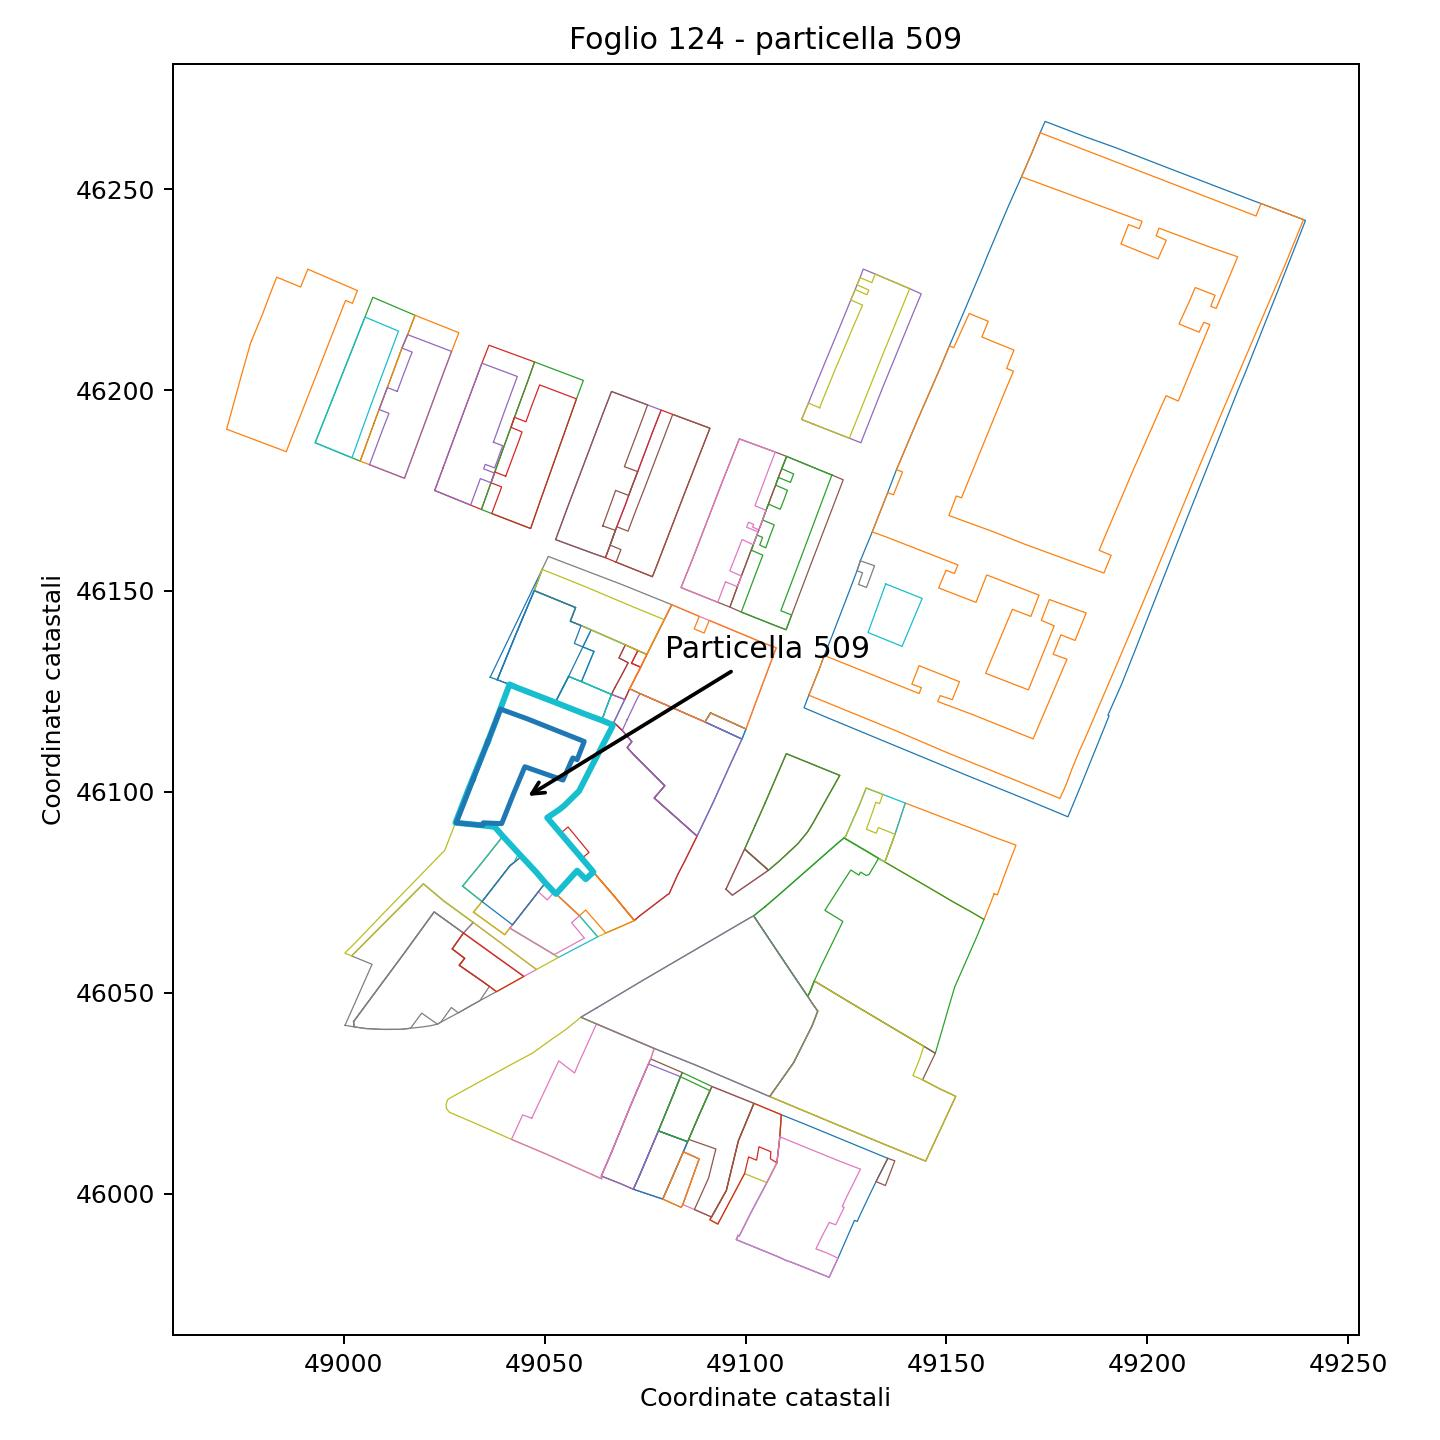
\includegraphics[width=.88\textwidth]{figures/particella-509-dxf.jpg}
\caption{Estratto del foglio catastale originario 124: localizzazione della particella 509 e del sedime storico.}\end{figure}}{}

Il DXF resta importante per confrontare il sedime originario con ortofoto e cartografia attuale e verificare se l'ingombro esterno nella zona veranda/bagno fosse già presente.

\section{PRG, Gran Camposanto e fascia cimiteriale}
La particella 509 è molto vicina al Gran Camposanto. Nel Geoportale comunale sono stati individuati il PRG, la zona cimiteriale H3 e servizi cartografici relativi ai vincoli, fra cui una categoria fascia cimiteriale.
\openq{Non è ancora dimostrato che la particella 509 ricada nella fascia di rispetto. Una linea/poligono visibile passa in prossimità dell'area, ma senza interrogazione puntuale del layer non costituisce prova.}

\section{Matrice delle evidenze}
\begin{tabularx}{\textwidth}{p{4cm}p{2.6cm}X}\toprule
\textbf{Elemento}&\textbf{Stato}&\textbf{Valore / limite}\\\midrule
Identificativi sub 5 & Documentato & Certi catastalmente; non provano conformità edilizia.\\
Nuova costruzione 11/12/1963 & Documentato & Forte riferimento cronologico; non è il titolo comunale.\\
Planimetria 1965 & Documentato & Riferimento geometrico storico.\\
Nessuna variazione interna sub 5 dal 1987 & Documentato & Nessun DOCFA recente emerso per ampliamento/distribuzione.\\
Modifica bagno precedente al 2005 & Ricordo & Da corroborare documentalmente.\\
Sub 32 ampliato nel 2013 & Documentato & Modifica individuale successiva; non spiega da sola il sub 5.\\
Sub 12 con planimetria 1965 & Documentato & Confronto utile se sovrapposto al sub 5.\\
Sedime storico DXF & Documentato & Utile per sagoma esterna, non per interni/subalterni.\\
Fascia cimiteriale su p. 509 & Aperto & Da verificare con interrogazione puntuale e atti.\\
Titolo edilizio originario & Aperto & Da reperire online o con accesso agli atti.\\
\bottomrule\end{tabularx}

\section{Prossimi passi}
\begin{enumerate}[leftmargin=*]
\item Ottenere l'\textbf{elaborato planimetrico} della particella 509 per identificare la colonna verticale del sub 5.
\item Confrontare la planimetria 1965 del sub sovrapposto con quella del sub 5.
\item Confrontare il DXF originario con ortofoto storiche regionali.
\item Interrogare puntualmente i layer Carta Vincoli Sovraordinati, PRG e fascia cimiteriale.
\item Cercare online atti su Gran Camposanto, fascia di rispetto, eventuali riduzioni, particella 509 e Via Bufalini.
\item Solo dopo, predisporre un \textbf{accesso agli atti mirato}: titolo/progetto originario circa 1963, varianti, sanatorie/condoni, agibilità/abitabilità, eventuali pratiche condominiali e atti sulla fascia cimiteriale.
\end{enumerate}

\section{Nota metodologica}
Il dossier non è una relazione tecnica asseverata né una certificazione dello stato legittimo. È uno strumento incrementale per organizzare le evidenze, distinguere fatti da ricordi e ipotesi, evitare duplicazioni e preparare richieste mirate agli uffici o a un tecnico incaricato.
\end{document}
